%!Mode:: "TeX:UTF-8"
\documentclass[a4paper,11pt,UTF8]{ctexart}

\usepackage{indentfirst} %缩进
\usepackage{xeCJK}    %使用系统字体
\usepackage{fancyhdr} %自定义页眉页脚
\pagestyle{empty}                   %不设置页眉页脚
\usepackage{amsmath, amsthm, amssymb, amsfonts} %数学公式
\usepackage[a4paper,left=3cm,right=3cm,top=3cm,bottom=3cm]{geometry}
%\usepackage[tmargin=1in,bmargin=1in,lmargin=1.25in,rmargin=1.25in]{geometry}.
\usepackage{booktabs} %插入表格
\usepackage[section]{placeins} %避免浮动
\usepackage{listings} %插入代码
\usepackage{ctex}     %中文宏包
\usepackage[svgnames, table]{xcolor} %彩色表格
\usepackage{algorithm}          %伪代码
\usepackage{algorithmicx}
\usepackage{algpseudocode}
\usepackage{algorithm,algpseudocode,float}
\usepackage{lipsum}
\usepackage{enumitem}           %调整列举环境
\usepackage{url}
\usepackage{fontspec,xunicode}
\defaultfontfeatures{Mapping=tex-text} %如果没有它,会有一些 tex 特殊字符无法正常使用,比如连字符。

\usepackage{graphicx}
\graphicspath{{imgs/}}
\usepackage{physics}
%%%%%%%%%%%%%%%%%%%%%%%%%%%%%%%%%%%%%%%%%%%%%%%%%%%%%%%%%%%%%%%%
% 缩进及行间距
%%%%%%%%%%%%%%%%%%%%%%%%%%%%%%%%%%%%%%%%%%%%%%%%%%%%%%%%%%%%%%%%
\setlength{\parindent}{0pt} %重新定义缩进长度
\setlength{\baselineskip}{20pt}  %定义行间距
%\renewcommand{\baselinestretch}{1.1} %定义行间距

%%%%%%%%%%%%%%%%%%%%%%%%%%%%%%%%%%%%%%%%%%%%%%%%%%%%%%%%%%%%%%%%
% 列表设置
%%%%%%%%%%%%%%%%%%%%%%%%%%%%%%%%%%%%%%%%%%%%%%%%%%%%%%%%%%%%%%%%
\setenumerate{fullwidth,itemindent=\parindent,listparindent=\parindent,itemsep=0ex,partopsep=0pt,parsep=0ex}
\setenumerate[2]{label=\alph*),leftmargin=1.5em}  %二级item设置
\setitemize{itemindent=38pt,leftmargin=0pt,itemsep=-0.4ex,listparindent=26pt,partopsep=0pt,parsep=0.5ex,topsep=-0.25ex}
\setdescription{itemindent=38pt,leftmargin=0pt,itemsep=-0.4ex,listparindent=26pt,partopsep=0pt,parsep=0.5ex,topsep=-0.25ex}

%%%%%%%%%%%%%%%%%%%%%%%%%%%%%%%%%%%%%%%%%%%%%%%%%%%%%%%%%%%%%%%%
% 图的标题行间距设置
%%%%%%%%%%%%%%%%%%%%%%%%%%%%%%%%%%%%%%%%%%%%%%%%%%%%%%%%%%%%%%%%
\newcommand{\bottomcaption}{%
\setlength{\abovecaptionskip}{6pt}%
\setlength{\belowcaptionskip}{6pt}%
\caption}


%%%%%%%%%%%%%%%%%%%%%%%%%%%%%%%%%%%%%%%%%%%%%%%%%%%%%%%%%%%%%%%%
% 字体定义
%%%%%%%%%%%%%%%%%%%%%%%%%%%%%%%%%%%%%%%%%%%%%%%%%%%%%%%%%%%%%%%%
\setmainfont{Times New Roman}  %默认英文字体.serif是有衬线字体sans serif无衬线字体
\setmonofont{Consolas}
\setCJKmainfont[ItalicFont={楷体}, BoldFont={黑体}]{宋体}%衬线字体 缺省中文字体为
\setCJKsansfont{黑体}
\punctstyle{hangmobanjiao}
%-----------------------xeCJK下设置中文字体------------------------------%
\setCJKfamilyfont{song}{SimSun}                             %宋体 song
\newcommand{\song}{\CJKfamily{song}}
\setCJKfamilyfont{fs}{FangSong}                      %仿宋  fs
\newcommand{\fs}{\CJKfamily{fs}}
\setCJKfamilyfont{ktgb}{KaiTi}                      %楷体2312 ktgb
\newcommand{\ktgb}{\CJKfamily{ktgb}}
\setCJKfamilyfont{yh}{Microsoft YaHei}                    %微软雅黑 yh
\newcommand{\yh}{\CJKfamily{yh}}
\setCJKfamilyfont{hei}{SimHei}                              %黑体  hei
\newcommand{\hei}{\CJKfamily{hei}}
\setCJKfamilyfont{hwxk}{STXingkai}                                %华文行楷  hwxk
\newcommand{\hwxk}{\CJKfamily{hwxk}}
%------------------------------设置字体大小------------------------%
\newcommand{\shiyanbaogao}{\fontsize{36pt}{\baselineskip}\selectfont}
\newcommand{\chuhao}{\fontsize{42pt}{\baselineskip}\selectfont}     %初号
\newcommand{\xiaochuhao}{\fontsize{36pt}{\baselineskip}\selectfont} %小初号
\newcommand{\yihao}{\fontsize{28pt}{\baselineskip}\selectfont}      %一号
\newcommand{\erhao}{\fontsize{21pt}{\baselineskip}\selectfont}      %二号
\newcommand{\xiaoerhao}{\fontsize{18pt}{\baselineskip}\selectfont}  %小二号
\newcommand{\sanhao}{\fontsize{15.75pt}{\baselineskip}\selectfont}  %三号
\newcommand{\sihao}{\fontsize{14pt}{\baselineskip}\selectfont}       %四号
\newcommand{\xiaosihao}{\fontsize{12pt}{\baselineskip}\selectfont}  %小四号
\newcommand{\wuhao}{\fontsize{10.5pt}{\baselineskip}\selectfont}    %五号
\newcommand{\xiaowuhao}{\fontsize{9pt}{\baselineskip}\selectfont}   %小五号
\newcommand{\liuhao}{\fontsize{7.875pt}{\baselineskip}\selectfont}  %六号
\newcommand{\qihao}{\fontsize{5.25pt}{\baselineskip}\selectfont}    %七号

%%%%%%%%%%%%%%%%%%%%%%%%%%%%%%%%%%%%%%%%%%%%%%%%%%%%%%%%%%%%%%%%
% 图题字体大小相同
%%%%%%%%%%%%%%%%%%%%%%%%%%%%%%%%%%%%%%%%%%%%%%%%%%%%%%%%%%%%%%%%
\usepackage{caption}
\captionsetup{font={footnotesize}}   % footnotesize = 9pt
\captionsetup[lstlisting]{font={footnotesize}}

%%%%%%%%%%%%%%%%%%%%%%%%%%%%%%%%%%%%%%%%%%%%%%%%%%%%%%%%%%%%%%%%
% 重定义枚举编号为 1),2)...
%%%%%%%%%%%%%%%%%%%%%%%%%%%%%%%%%%%%%%%%%%%%%%%%%%%%%%%%%%%%%%%%
\renewcommand{\labelenumi}{\theenumi)}

%%%%%%%%%%%%%%%%%%%%%%%%%%%%%%%%%%%%%%%%%%%%%%%%%%%%%%%%%%%%%%%%
% 标题名称中文化
%%%%%%%%%%%%%%%%%%%%%%%%%%%%%%%%%%%%%%%%%%%%%%%%%%%%%%%%%%%%%%%%
\renewcommand\figurename{\hei 图}
\renewcommand\tablename{\hei 表}
\renewcommand\lstlistingname{\hei 代码}
\renewcommand{\algorithmicrequire}{\textbf{输入:}}
\renewcommand{\algorithmicensure}{\textbf{输出:}}
\newtheorem{define}{定义}

%%%%%%%%%%%%%%%%%%%%%%%%%%%%%%%%%%%%%%%%%%%%%%%%%%%%%%%%%%%%%%%%
% 代码设置
%%%%%%%%%%%%%%%%%%%%%%%%%%%%%%%%%%%%%%%%%%%%%%%%%%%%%%%%%%%%%%%%
\lstset{
 columns=fixed,
 numbers=left,                                        % 在左侧显示行号
 numberstyle=\tiny\color{gray},                       % 设定行号格式
 frame=single,                                        % 单线背景边框
 breaklines=true,                                     % 设定LaTeX对过长的代码行进行自动换行
 keywordstyle=\color[RGB]{40,40,255},                 % 设定关键字颜色
 numberstyle=\footnotesize\color{darkgray},
 commentstyle=\it\color[RGB]{0,96,96},                % 设置代码注释的格式
 stringstyle=\rmfamily\slshape\color[RGB]{128,0,0},   % 设置字符串格式
 showstringspaces=false,                              % 不显示字符串中的空格
 language=java,                                        % 设置语言
 basicstyle=\linespread{1.0}\xiaowuhao\ttfamily,                      % 字体字号
 %lineskip=10pt,
 %baselinestretch=1,
}

%%%%%%%%%%%%%%%%%%%%%%%%%%%%%%%%%%%%%%%%%%%%%%%%%%%%%%%%%%%%%%%%
% 伪代码分页
%%%%%%%%%%%%%%%%%%%%%%%%%%%%%%%%%%%%%%%%%%%%%%%%%%%%%%%%%%%%%%%%
\makeatletter
\renewcommand{\ALG@name}{算法}
\newenvironment{breakablealgorithm}
  {% \begin{breakablealgorithm}
   \begin{center}
     \refstepcounter{algorithm}% New algorithm
     \hrule height.8pt depth0pt \kern2pt% \@fs@pre for \@fs@ruled
     \renewcommand{\caption}[2][\relax]{% Make a new \caption
       {\raggedright\textbf{\ALG@name~\thealgorithm} ##2\par}%
       \ifx\relax##1\relax % #1 is \relax
         \addcontentsline{loa}{algorithm}{\protect\numberline{\thealgorithm}##2}%
       \else % #1 is not \relax
         \addcontentsline{loa}{algorithm}{\protect\numberline{\thealgorithm}##1}%
       \fi
       \kern2pt\hrule\kern2pt
     }
  }{% \end{breakablealgorithm}
     \kern2pt\hrule\relax% \@fs@post for \@fs@ruled
   \end{center}
  }
\makeatother

% =============================================
% Part 1 Edit the info
% =============================================


\newcommand{\course}{电子线路实验(1)}
\newcommand{\newtitle}{数据选择器}

\title{数据选择器}
\author{PB19000132苗立扬  PB18020556 戴佳乐}

% =============================================
% Part 1 Main document
% =============================================
\begin{document}


% =============================================
% Part 2 Main document
% =============================================

%
\newcommand{\p}{\par}
\newcommand{\np}{\par\noindent}
%
\newcommand{\expa}{验证4选1数据选择器74LS153的逻辑功能并记录真值表}
\newcommand{\expb}{验证8选1数据选择器74LS151的逻辑功能并记录真值表}
\newcommand{\expc}{用两个8选1数据选择器74LS151扩展成16选1数据选择器,实现逻辑函数$Y=\sum m(6,7,8,11,13)$画出简图并记录真值表}
\newcommand{\expd}{用双4选1数据选择器74LS153实现一位全加器}
\newcommand{\chip}{数据选择器74LS151}

\newcommand{\CI}{C\negthinspace I}
\newcommand{\CO}{C\negthinspace O}
%

\maketitle

\section{实验目的}

(1)熟悉中规模集成电路数据选择器的工作原理和逻辑功能。\\
(2)了解数据选择器的应用。\\


\section{实验原理}

(1)数据选择器又称多路选择器,是一个数据开关,它从N路源数据中选择一路送至输出端。
\\
(2)双4选1数据选择器74LS153。
\begin{figure}[H]
  \centering
  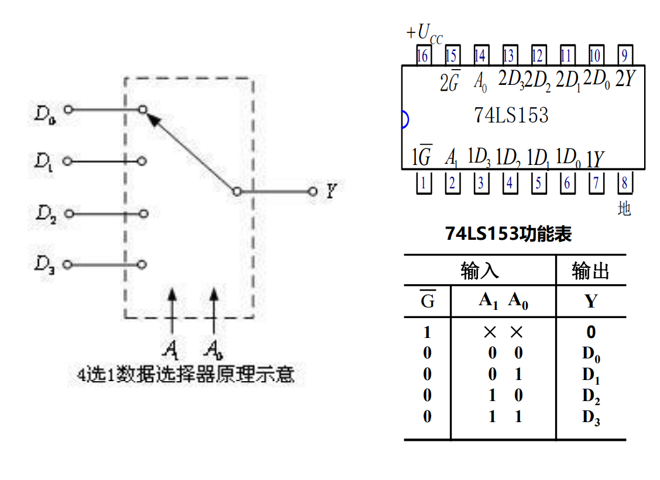
\includegraphics[width=12cm]{new01}
  \caption{74LS153}
  \label{fig:new01}
\end{figure}
(3)74LS151是8选1数据选择器,三个控制端A0、A1、A2,
有8种组合,000、001、010、011、100、101、110、
111。
\begin{figure}[H]
  \centering
  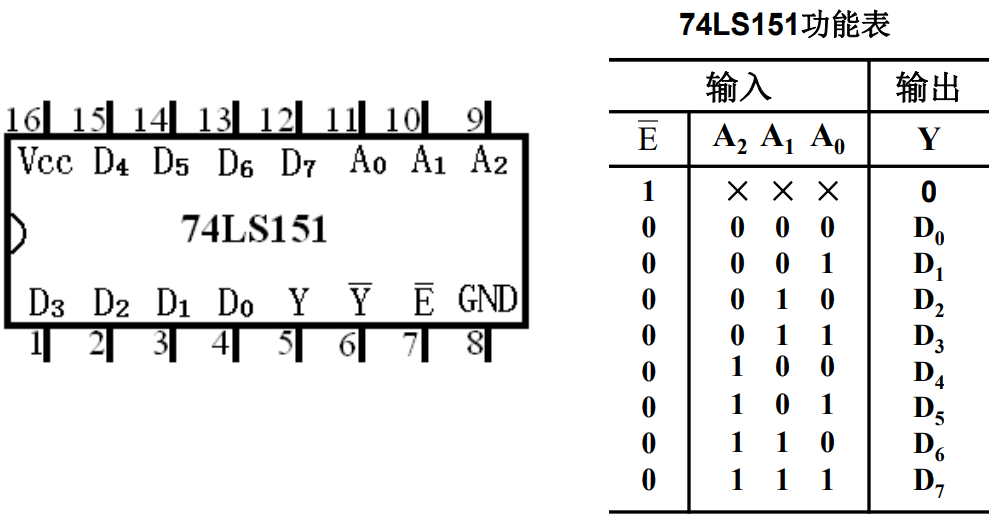
\includegraphics[width=14cm]{new02}
  \caption{74LS151}
  \label{fig:new01}
\end{figure}

\section{实验内容、步骤与结果}
 \subsection{实验一:\expa}
 \begin{table}[H]
  \centering
  \begin{tabular}{|ccccccc|c|}\hline
   \multicolumn{7}{|c|}{输入}  &输出
   \\\hline
   $\bar{G}$ &$A_1$ &$A_0$ &$D_3$ &$D_2$ &
   $D_1$ &$D_0$  &$Y$
   \\\hline
   1 &$\times$ &$\times$ &$\times$	&$\times$ &$\times$ &$\times$ &0	\\
   0 &0 &0 &$\times$	&$\times$ &$\times$ &$\smqty{0\\1}$ &$\smqty{0\\1}$	\\
   0 &0 &1 &$\times$	&$\times$ &$\smqty{0\\1}$ &$\times$ &$\smqty{0\\1}$	\\
   0 &1 &0 &$\times$	&$\smqty{0\\1}$ &$\times$ &$\times$ &$\smqty{0\\1}$	\\
   0 &1 &1 &$\smqty{0\\1}$	&$\times$ &$\times$ &$\times$ &$\smqty{0\\1}$	
   \\\hline
  \end{tabular}
  \caption{实验一真值表}
  \label{tab:Exp01}
 \end{table}
 \subsection{实验二:\expb}
 \begin{table}[H]
  \centering
  \begin{tabular}{|cccccccccccc|c|}\hline
   \multicolumn{12}{|c|}{输入}  &输出
   \\\hline
   $\bar{E}$ &$A_2$ &$A_1$ &$A_0$ &$D_7$ &
   $D_6$ &$D_5$ &$D_4$ &$D_3$ &$D_2$ &$D_1$ &$D_0$ &$Y$
   \\\hline
   1 &$\times$ &$\times$ &$\times$	&$\times$ &$\times$ &$\times$ &$\times$ &$\times$ &$\times$ &$\times$ &$\times$ &0	\\
   0 &0 &0 &0 &$\times$ &$\times$ &$\times$ &$\times$ &$\times$ &$\times$ &$\times$ &$\smqty{0\\1}$ &$\smqty{0\\1}$	\\
   0 &0 &0 &1 &$\times$ &$\times$ &$\times$ &$\times$ &$\times$ &$\times$ &$\smqty{0\\1}$ &$\times$ &$\smqty{0\\1}$	\\
   0 &0 &1 &0 &$\times$ &$\times$ &$\times$ &$\times$ &$\times$ &$\smqty{0\\1}$ &$\times$ &$\times$ &$\smqty{0\\1}$	\\
   0 &0 &1 &1 &$\times$ &$\times$ &$\times$ &$\times$ &$\smqty{0\\1}$	&$\times$ &$\times$ &$\times$ &$\smqty{0\\1}$	\\
   0 &1 &0 &0 &$\times$ &$\times$ &$\times$ &$\smqty{0\\1}$ &$\times$ &$\times$ &$\times$ &$\times$ &$\smqty{0\\1}$  \\
   0 &1 &0 &1 &$\times$ &$\times$ &$\smqty{0\\1}$ &$\times$ &$\times$ &$\times$ &$\times$ &$\times$ &$\smqty{0\\1}$  \\
   0 &1 &1 &0 &$\times$ &$\smqty{0\\1}$ &$\times$ &$\times$ &$\times$ &$\times$ &$\times$ &$\times$ &$\smqty{0\\1}$  \\
   0 &1 &1 &1 &$\smqty{0\\1}$ &$\times$ &$\times$ &$\times$ &$\times$ &$\times$ &$\times$ &$\times$ &$\smqty{0\\1}$  
   \\\hline
  \end{tabular}
  \caption{实验二真值表}
  \label{tab:Exp02}
 \end{table}
  
 \subsection{实验三:\expc}
 
 \begin{figure}[H]
  \centering
  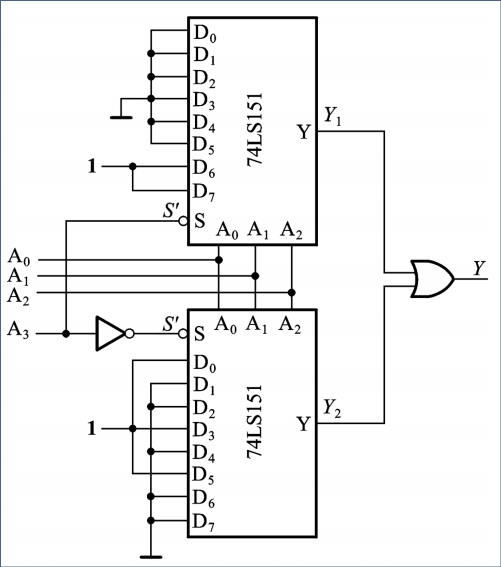
\includegraphics[width=10cm]{Exp02}
  \caption{实验三电路图}
  \label{fig:Exp03}
 \end{figure}

 \begin{table}[H]
  \centering
  \begin{tabular}{|cccc|c|cccc|c|}\hline
   \multicolumn{4}{|c|}{输入} &输出 
   &\multicolumn{4}{|c|}{输入} &输出
   \\\hline
   $A_3$ &$A_2$ &$A_1$ &$A_0$ &$Y$ &
   $A_3$ &$A_2$ &$A_1$ &$A_0$ &$Y$
   \\\hline
   0 &0 &0 &0	&0 &
   1 &0 &0 &0	&1\\
   0 &0 &0 &1	&0 &
   1 &0 &0 &1	&0\\
   0 &0 &1 &0	&0 &
   1 &0 &1 &0	&0\\
   0 &0 &1 &1	&0 &
   1 &0 &1 &1	&1\\
   0 &1 &0 &0	&0 &
   1 &1 &0 &0	&0\\
   0 &1 &0 &1	&0 &
   1 &1 &0 &1	&1\\
   0 &1 &1 &0	&1 &
   1 &1 &1 &0	&0\\
   0 &1 &1 &1	&1 &
   1 &1 &1 &1	&0
   \\\hline
  \end{tabular}
  \caption{实验三真值表}
  \label{tab:Exp03}
 \end{table}

  
 

\section{总结}
通过这次实验,本组同学熟悉了中规模集成电路数据选择器的工作原理和逻辑功能,了解了数据选择器的应用。
\\
本次实验我们使用了数据选择器。8 选 1 数据选择器 74LS151 有 3 位地址位和 8 位输入,两个8选1数据选择器74LS151可以扩展成16选1数据选择器,因此可以构造四个变量的任意逻辑函数。

 

\end{document}
